
\chapter{Modèle mémoire E-ACSL}
\label{sec:eacsl}

\chapterintro


Dans ce chapitre nous présentons notre implémentation du modèle mémoire en C
qui permet d'exécuter les annotations \eacsl présentées dans
le chapitre~\ref{sec:runtime}.
Notre bibliothèque permet au greffon \eacsltoc de vérifier à l'exécution les
annotations \eacsl portant sur le modèle mémoire.

\eacsltoc traduit automatiquement un programme C annoté en un autre
programme dont l'exécution échouera si une annotation n'est pas valide.
Si aucune annotation n'est violée, le comportement
du nouveau programme est exactement le même que celui du programme d'origine.
Ce greffon utilise notre bibliothèque afin de vérifier à l'exécution les
annotations \eacsl portant sur le modèle mémoire.

Nous présentons la bibliothèque en partie~\ref{sec:eacsl-impl} et les résultats
de nos expérimentations en partie~\ref{sec:eacsl-exp}.


\section{Implémentation}
\label{sec:eacsl-impl}


\begin{landscape}
  \begin{figure}[tb]
    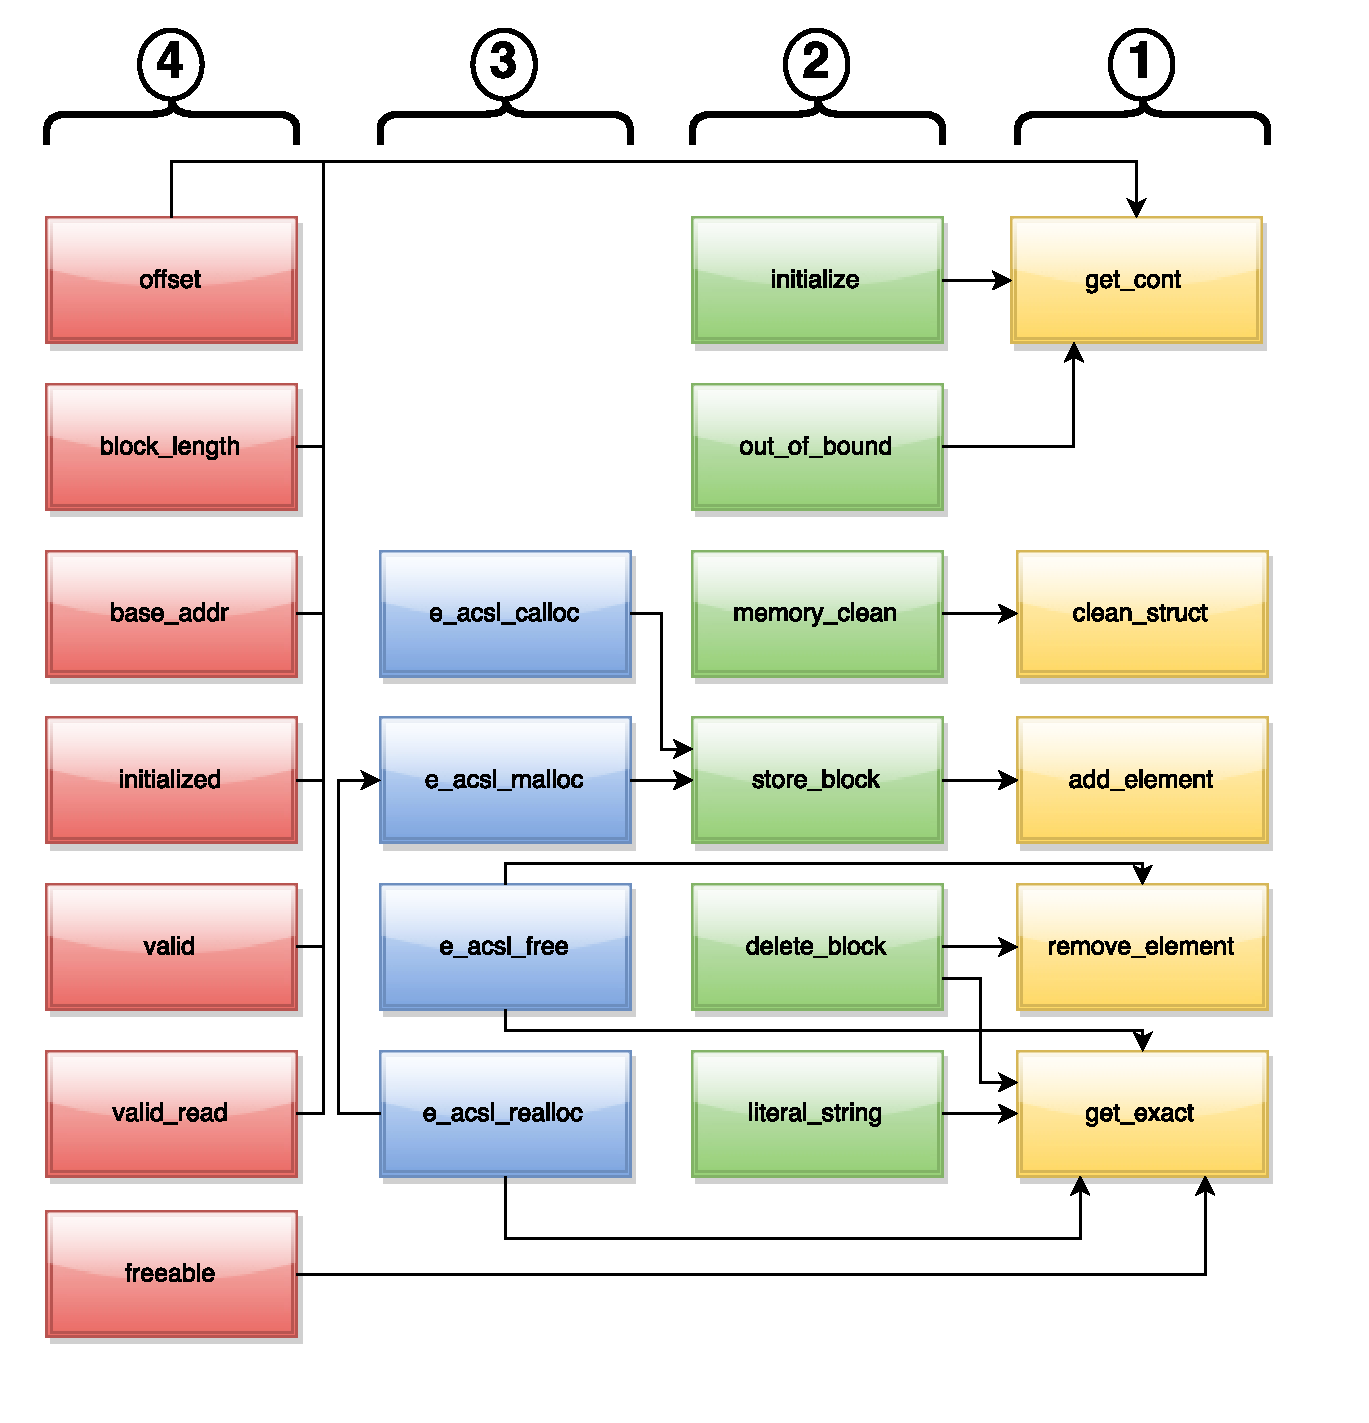
\includegraphics{figures/mmodel_architecture.pdf}
    \label{fig:mmodel-architecture}
    \caption{Architecture de la bibliothèque de modèle mémoire d'\eacsl}
  \end{figure}
\end{landscape}


\section{Expérimentations}
\label{sec:eacsl-exp}


Pour évaluer notre solution, nous avons effectué plus de 300 exécutions sur
plus de 30 programmes, obtenus à partir d'une dizaine d'exemples. Nous avons
volontairement gardés des exemples plutôt courts (moins de 200 lignes de code)
car ils ont dû être annotés en \acsl manuellement.

Nous avons mesuré le temps d'exécution du programme d'origine et du code
instrumenté par \eacsltoc avec différentes options, afin d'évaluer les
performances des différentes implémentations et optimisations. Des indicateurs
comme le nombre de variables, d'allocations mémoires, d'enregistrements et de
requêtes a également été enregistré.



\textbf{Implémentation du store :}\\
Pour déterminer quelle implémentation du $store$ est la plus appropriée, nous
avons comparé des implémentations utilisant : des Patricia tries, des listes
chaînées, des arbres binaires de recherche non équilibrés et des Splay trees.

Notre implémentation utilisant les Patricia tries est en moyenne 2500 fois plus
rapide que l'implémentation à base de listes chaînées, 200 fois plus rapide que
celle utilisant les arbres binaires de recherche, et 27 fois plus rapide que
celle se basant sur les Splay trees.

La version utilisant les Splay trees offre
des performances comparables (ou légèrement meilleures, jusqu'à 3 fois) sur les
exemples contenant de fréquents accès mémoire consécutifs au même bloc dans le
$store$. En revanche, sur des examples où les accès méoire consécutifs ne se
font pas sur le même bloc (une multiplication de matrices dans notre exemple),
les performances sont beaucoup moins bonnes (jusqu'à 500 fois). Ceci est dû à
la nature des Splay treees : le dernier élément accédé est remonté à la racine
de l'arbre.

\textbf{Calcul du plus grand préfixe commun :} \\
Nous avons comparé deux implémentations de ce calcul. La première utilise un
parcours linéaire de l'adresse (bit-à-bit, de gauche à droite). La seconde
est une recherche dichotomique du meilleur préfixe dans un tableau dont le
contenu et les indices (indiquant le prochain élément à tester) sont
pré-calculés. Cette seconde implémentation s'est révélée en moyenne 2.7 fois
plus rapide que la première sur nos exemples.

\textbf{Capacité de détection d'erreurs :} \\
Nous avons utilisé le ``test mutationnel'' pour évaluer la capacité de détection
d'erreurs en utilisant la vérification d'assertion à l'exécution avec
\framac. Nous avons considéré 5 exemples annotés et généré leurs
{\em mutants} (en appliquant une {\em mutation} sur leur code source) et leur
avons appliqué la vérification à l'exécution. Les mutations incluent :
modifications d'opérateur arithmétique numérique, modifications d'opérateur
arithmétique sur les pointeurs, modifications d'opérateur de comparaison et
modifications d'opérateur logique ($land$ et $lor$).
L'outil de génération de test \pathcrawler \cite{\citepathcrawler} a été
utilisé pour produire les cas de test. Chaque mutant a été instrumenté par
\eacsltoc et exécuté sur chaque cas de test pour vérifier que la
spécification était satisfaite à l'exécution. Les programmes d'origine passent
toutes les vérifications à l'exécution. Lorsqu'une violation d'une annotation a
été reportée pour au moins un cas de testn le mutant est considéré comme étant
{\em tué}. La Table~\ref{tab:mutation-exp} illustre les résultats. Exception
faite des mutants équivalents (lorsque la mutation produit un programme
équivalent au programme d'origine), tous les mutants erronés ont été tués.


La Table~\ref{tab:mmodel-exp} contient les résultats des expérimentations
comparant les différentes implémentations du $store$ et du calcul du plus grand
préfixe commun, la Fig.~\ref{fig:mmodel-exp} représente graphiquement ces
données. bS$_{10000}$ est une recherche binaire dans un tableaux de 10000
éléments. iS$_{10000}$ est un tri par insertion d'un tableau de 10000 éléments.
mM$_{n^2}$ est une multiplication de matrices $n \times n$. mI$_{n^2}$ contient
des calculs matriciels (dont inversion et multiplication) sur des  matrices
$n \times n$. qS$_n$ est un tri rapide sur un tableau de $n$ éléments.
bbS$_{10000}$ est un tri à bulles sur un tableau à 10000 éléments. m$_{30000}$ est
une fusion de deux listes chaînées de 10000 et 20000 éléments. Rbt$_{10000}$ est
une insertion/suppression de 10000 éléments dans un arbre rouge et noir. mS$_n$
est un tri fusion d'une liste chaînée de $n$ éléments. La ligne supplémentaire
``+ RTE'' de chaque exemple correspond à une application préalable du greffon
\rte qui génère des assertions qui sont vraies si le programme ne
contient pas d'erreur à l'exécution.

Les colonnes ont la signification suivante : \danger{} contient le nombre
d'alarmes du programme,  $\emptyset$ contient le temps d'exécution du programme
original, bst correspond à l'implémentation par arbres binaires de recherche,
mask est le nombre de fois qu'est effectué le calcul du plus grand préfixe
commun, sb est le nombre d'insertion dans le $store$, Pt correspond à
l'implémentation par Patricia tries, St correspond à l'implémentation par Splay
trees. L'exposant $^1$ (respectivement $^2$) correspond aux expérimentations
sans (resp. avec) application d'une analyse statique $Dataflow$ permettant de
n'instrumenter que ce qui est nécessaire (section 6 de \cite{\citeeacsltoc}).
L'indice $_1$ (resp. $_2$)
correspond à l'implémentation non optimisée (resp. optimisée) du calcul du
plus grand préfixe commun pour l'implémentation utilisant les Patricia tries.
Le temps d'analyse du programme avec \valgrind \cite{\citevalgrind} est
indiqué dans la dernière colonne.

Nous remarquons que le temps d'exécution de \valgrind n'est pas
comparable avec celui de notre solution, cela s'explique simplement par le fait
que celui-ci ne prend pas en compte la spécification \acsl, et se
contente de vérifier des propriétés comme l'absence d'erreur de segmentation ou
l'absence de fuite de mémoire. En revanche, notre démarche vise à supporter au
maximum les annotations \acsl, ce qui nécessite un monitoring plus
lourd.

Nos expérimentations, présentées dans la Fig.~\ref{fig:mmodel-exp}, confirment
nos hypothèses, à savoir :
\begin{itemize}
\item le Patricia trie est la structure de données la plus appropriée pour
  l'implémentation du $store$;
\item notre optimisation du calcul du plus grand préfixe commun par recherche
  dichotomique et utilisation d'indices pré-calculés entraîne un vrai gain de
  performance;
\item l'utilisation d'une analyse statique visant à réduire l'instrumentation
  du programme permet de réduire le temps d'exécution de manière efficace.
\end{itemize}


\begin{landscape}
  \begin{table}[h]
    \centering
    \begin{footnotesize}
    \begin{tabular}{l|c|c|c|c|c|c|c|HHc|c|HHc|c|c|c}
  & $\danger$ & $\emptyset$ & list & list-AS & bst & bst-AS & Pt & mask$^1$ & sb$^1$ & Pt-dicho & Pt-AS & mask$^2$ & sb$^2$ & Pt-dicho-AS & St & St-AS & valgrind \\
  \hline
  bS$_{10000}$ &22 &\multirow{2}{*}{.01} &1.10 &0.50 &1.14 &0.64 &1.55 &99 &16 &1.55 &0.57 &0 &1 &0.55 &1.39 &0.61 &\multirow{2}{*}{0.27}\\
  + RTE &41 &&1.10 &0.51 &1.14 &0.62 &1.59 &109 &16 &1.59 &0.53 &0 &1 &0.53 &1.39 &0.64 &\\
  \hline
  iS$_{10000}$ &5 &\multirow{2}{*}{.12} &2.29 &0.12 &1.83 &0.12 &2.89 &170k &20k &2.91 &0.12 &0 &0 &0.12 &2.46 &0.12 &\multirow{2}{*}{2.81}\\
  + RTE &24 &&3.52 &1.27 &2.89 &1.26 &3.99 &170k &20k &3.86 &1.25 &0 &0 &1.25 &3.46 &1.30 &\\
  \hline
  mM$_{100^2}$ &0 &\multirow{2}{*}{.01} &2.29 &0.73 &2.94 &1.15 &0.14 &17k &1k &0.14 &0.10 &5k &612 &0.09 &1.07 &0.98 &\multirow{2}{*}{0.34}\\
  + RTE &82 &&13.17 &10.66 &21.92 &17.39 &2.78 &18k &1k &3.00 &2.64 &5k &612 &2.82 &75.97 &73.62 &\\
  \hline
  mM$_{150^2}$ &0 &\multirow{2}{*}{.01} &13.23 &3.96 &15.65 &6.20 &0.54 &21k &2k &0.51 &0.36 &9k &912 &0.35 &5.86 &5.64 &\multirow{2}{*}{0.48}\\
  + RTE &82 &&72.36 &58.48 &110.70 &90.43 &10.77 &24k &2k &9.01 &8.57 &9k &912 &8.75 &403.50 &398.60 &\\
  \hline
  mI$_{100^2}$ &2 &\multirow{2}{*}{.01} &22.51 &0.10 &7.74 &0.13 &0.09 &68k &5k &0.08 &0.01 &7k &609 &0.01 &0.19 &0.10 &\multirow{2}{*}{0.35}\\
  + RTE &155 &&28.96 &4.22 &13.67 &5.48 &0.54 &73k &5k &0.55 &0.53 &7k &611 &0.47 &26.37 &26.16 &\\
  \hline
  mI$_{150^2}$ &2 &\multirow{2}{*}{.02} &130.04 &0.34 &40.35 &0.45 &0.28 &99k &8k &0.27 &0.02 &12k &909 &0.02 &0.68 &0.34 &\multirow{2}{*}{0.47}\\
  + RTE &155 &&153.30 &21.54 &73.55 &29.94 &2.00 &105k &8k &1.90 &1.42 &12k &911 &1.53 &146.15 &145.80 &\\
  \hline
  qS$_{1000}$ &15 &\multirow{2}{*}{.01} &12.70 &2.08 &1.76 &0.59 &0.33 &1M &92k &0.06 &0.13 &683k &39k &0.02 &0.02 &0.01 &\multirow{2}{*}{0.27}\\
  + RTE &32 &&12.38 &2.13 &1.64 &0.56 &0.38 &1M &92k &0.12 &0.14 &727k &39k &0.04 &0.03 &0.02 &\\
  \hline
  qS$_{2000}$ &15 &\multirow{2}{*}{.01} &85.99 &11.31 &8.39 &2.78 &0.71 &3M &198k &0.14 &0.28 &1M &84k &0.05 &0.03 &0.02 &\multirow{2}{*}{0.27}\\
  + RTE &32 &&81.65 &11.15 &7.72 &2.67 &1.13 &4M &198k &0.48 &0.36 &1M &84k &0.13 &0.05 &0.02 &\\
  \hline
  bbS$_{10000}$ &4 &\multirow{2}{*}{.22} &13.78 &1.02 &16.84 &1.67 &117.47 &499M &49M &22.36 &1.57 &30 &7 &1.54 &8.80 &1.67 &\multirow{2}{*}{3.36}\\
  + RTE &16 &&23.08 &4.64 &30.69 &7.16 &107.05 &599M &49M &32.58 &7.26 &29 &7 &6.90 &17.29 &7.21 &\\
  \hline
  m$_{30000}$ &2 &\multirow{2}{*}{.01} &412.10 &11.38 &176.35 &11.01 &1.11 &5M &420k &0.26 &0.30 &1M &60k &0.06 &0.08 &0.01 &\multirow{2}{*}{0.45}\\
  + RTE &49 &&451.58 &101.33 &219.12 &94.80 &1.15 &5M &420k &0.29 &0.47 &2M &130k &0.14 &0.10 &0.05 &\\
  \hline
  Rbt$_{10000}$ &0 &\multirow{2}{*}{.01} &47.39 &0.28 &48.44 &0.27 &0.32 &1M &159k &0.09 &0.03 &151k &10k &0.01 &0.59 &0.01 &\multirow{2}{*}{0.51}\\
  + RTE &270 &&120.02 &101.69 &165.77 &145.20 &0.47 &1M &159k &0.30 &0.39 &979k &119k &0.27 &18.82 &19.59 &\\
  \hline
  mS$_{1000}$ &7 &\multirow{2}{*}{.01} &6.45 &0.34 &6.32 &0.11 &0.32 &1M &95k &0.07 &0.06 &331k &18k &0.01 &0.02 &0.01 &\multirow{2}{*}{0.27}\\
  + RTE &45 &&6.82 &1.35 &7.98 &0.38 &0.34 &1M &95k &0.10 &0.13 &701k &38k &0.04 &0.02 &0.01 &\\
  \hline
  mS$_{5000}$ &7 &\multirow{2}{*}{.01} &362.87 &11.00 &218.01 &3.43 &2.28 &11M &562k &0.76 &0.43 &2M &106k &0.09 &0.14 &0.03 &\multirow{2}{*}{0.27}\\
  + RTE &45 &&371.40 &50.94 &290.88 &10.34 &2.46 &11M &562k &0.80 &0.83 &4M &218k &0.22 &0.16 &0.08 &\\
  \hline
  mS$_{10000}$ &7 &\multirow{2}{*}{.01} &3624.01 &47.94 &1673.00 &16.10 &6.46 &23M &1M &2.75 &1.00 &5M &223k &0.21 &0.31 &0.08 &\multirow{2}{*}{0.27}\\
  + RTE &45 &&3406.43 &257.18 &2086.32 &46.22 &6.30 &23M &1M &2.66 &1.83 &9M &457k &0.51 &0.35 &0.18 &\\
  \hline
  mS$_{50000}$ &7 &\multirow{2}{*}{.01} &$\infty$ &3847.72 &$\infty$ &1100.93 &135.54 &146M &6M &111.22 &6.90 &33M &1M &1.65 &2.08 &0.58 &\multirow{2}{*}{0.63}\\
  + RTE &45 &&$\infty$ &25554.08 &$\infty$ &2781.90 &118.86 &145M &6M &95.74 &11.64 &54M &2M &3.37 &2.18 &1.15 &\\
  \hline
  mS$_{100000}$ &7 &\multirow{2}{*}{.01} &$\infty$ &$\infty$ &$\infty$ &$\infty$ &631.41 &296M &14M &559.93 &13.55 &70M &2M &3.35 &4.03 &1.15 &\multirow{2}{*}{0.27}\\
  + RTE &45 &&$\infty$ &$\infty$ &$\infty$ &$\infty$ &573.47 &308M &14M &513.85 &25.02 &116M &5M &7.63 &4.68 &2.50 &\\
\end{tabular}

    \end{footnotesize}
    \label{tab:mmodel-exp}
    \caption{Comparaison des différentes implémentations du $store$}
  \end{table}
\end{landscape}


\begin{figure}[bt]
  \begin{tikzpicture}
    \begin{axis}[axis y line=left,width=\textwidth,height=\textwidth,ymode=log]
      \pgfplotstableread{data/table_eacsl_experiments_merge_sort.dat}
      \loadedtable;
      \foreach \i in {
        list,list-DFA,bst,bst-DFA,Pt,Pt-opti,Pt-DFA,Pt-opti-DFA,St,St-DFA} {
        \addplot table [x=N, y=\i] {\loadedtable};
      }
      \legend{list,list-DFA,bst,bst-DFA,Pt,Pt-opti,Pt-DFA,Pt-opti-DFA,St,St-DFA}
    \end{axis}
  \end{tikzpicture}
  \label{fig:mmodel-exp}
  \caption{Comparaison des différentes implémentations du $store$}
\end{figure}


\begin{table}[tb]
  \centering
  \begin{tabular}{c|c|c|c|c|c}
    & alarmes & mutants & équivalents & tués & \% erronés tués \\
    \hline
    fibonacci & 19  & 27 & 2 & 25 & 100\% \\
    \hline
    bubbleSort & 15  & 44 & 2 & 42 & 100\% \\
    \hline
    insertionSort & 10  & 39 & 3 & 36 & 100\% \\
    \hline
    binarySearch & 7 & 38 & 1 & 37 & 100\% \\
    \hline
    merge & 5 & 92 & 5 & 87 & 100\% \\
  \end{tabular}
  \label{tab:mutation-exp}
  \caption{Capacité de détection d'erreurs}
\end{table}


\section*{Conclusion du chapitre}

TODO
